\chapter{Empujones y tirones: las fuerzas}\label{ch:g2:pushes-and-pulls}

Abrir una puerta, subir una cremallera, chutar un balón, arrastrar un
trineo: te pasas el día entero empujando y tirando. La física reúne
todo esto bajo un nombre orgulloso --- \omterm{def:g2:pushes-and-pulls:force}{fuerza} --- y hace dos preguntas
sencillas: ¿qué puede hacer una \omterm{def:g2:pushes-and-pulls:force}{fuerza} y hacia dónde actúa?

\section{Empujones y tirones por todas partes}

\begin{definition}[La fuerza]\label{def:g2:pushes-and-pulls:force}
Una \emph{fuerza}\index{fuerza} es un empujón o un tirón. Empujar un
columpio, tirar de un carrito, apretar un timbre, estirar una goma
elástica, amasar pan: en todos estos casos hay una fuerza trabajando.
Una fuerza tiene siempre una intensidad --- suave o tremenda --- y una
\emph{dirección}: empuja o tira \emph{hacia algún lado}.
\end{definition}

\begin{example}[¿Empujón o tirón?]\label{ex:g2:pushes-and-pulls:sort}
Clasifica tu día: chutar un balón --- un empujón con el pie. Abrir un
cajón --- un tirón. Cerrarlo --- un empujón. Subirse la cremallera de
la chaqueta --- un tirón. Amasar pan --- muchos empujoncitos. Tirar de la
cuerda --- dos equipos tirando de la misma soga en sentidos
contrarios.
\end{example}

\begin{method}[Dibujar una fuerza como una flecha]\label{met:g2:pushes-and-pulls:arrow}
Los físicos dibujan una \omterm{def:g2:pushes-and-pulls:force}{fuerza} como una \emph{flecha}:
\begin{enumerate}
  \item la flecha empieza donde el empujón o el tirón agarra el
        objeto;
  \item apunta hacia donde actúa la \omterm{def:g2:pushes-and-pulls:force}{fuerza};
  \item una \omterm{def:g2:pushes-and-pulls:force}{fuerza} más intensa lleva una flecha más larga.
\end{enumerate}
Una flechita cuenta la historia entera: dónde, hacia dónde y con
cuánta \omterm{def:g2:pushes-and-pulls:force}{fuerza}. Dibujaremos estas flechas durante muchos años.
\end{method}

\begin{omfigure}
\begin{tikzpicture}[scale=0.85]
  \draw[thick] (0,0) -- (4.6,0);
  \draw[thick, fill=omMeth, fill opacity=0.4] (1.4,0) rectangle (2.9,1.0);
  \draw[-Stealth, very thick, omThm] (0.2,0.5) -- (1.3,0.5);
  \node[below, font=\small] at (2.3,-0.25) {empujón suave: flecha corta};
  \draw[thick] (6.4,0) -- (11.0,0);
  \draw[thick, fill=omMeth, fill opacity=0.4] (8.4,0) rectangle (9.9,1.0);
  \draw[-Stealth, very thick, omThm] (6.5,0.5) -- (8.3,0.5);
  \node[below, font=\small] at (8.7,-0.25) {empujón tremendo: flecha larga};
\end{tikzpicture}

{\small La misma caja empujada dos veces. La flecha enseña dónde
agarra el empujón, hacia dónde actúa y --- por su longitud --- con
cuánta \omterm{def:g2:pushes-and-pulls:force}{fuerza}.}
\end{omfigure}

\begin{omfigure}
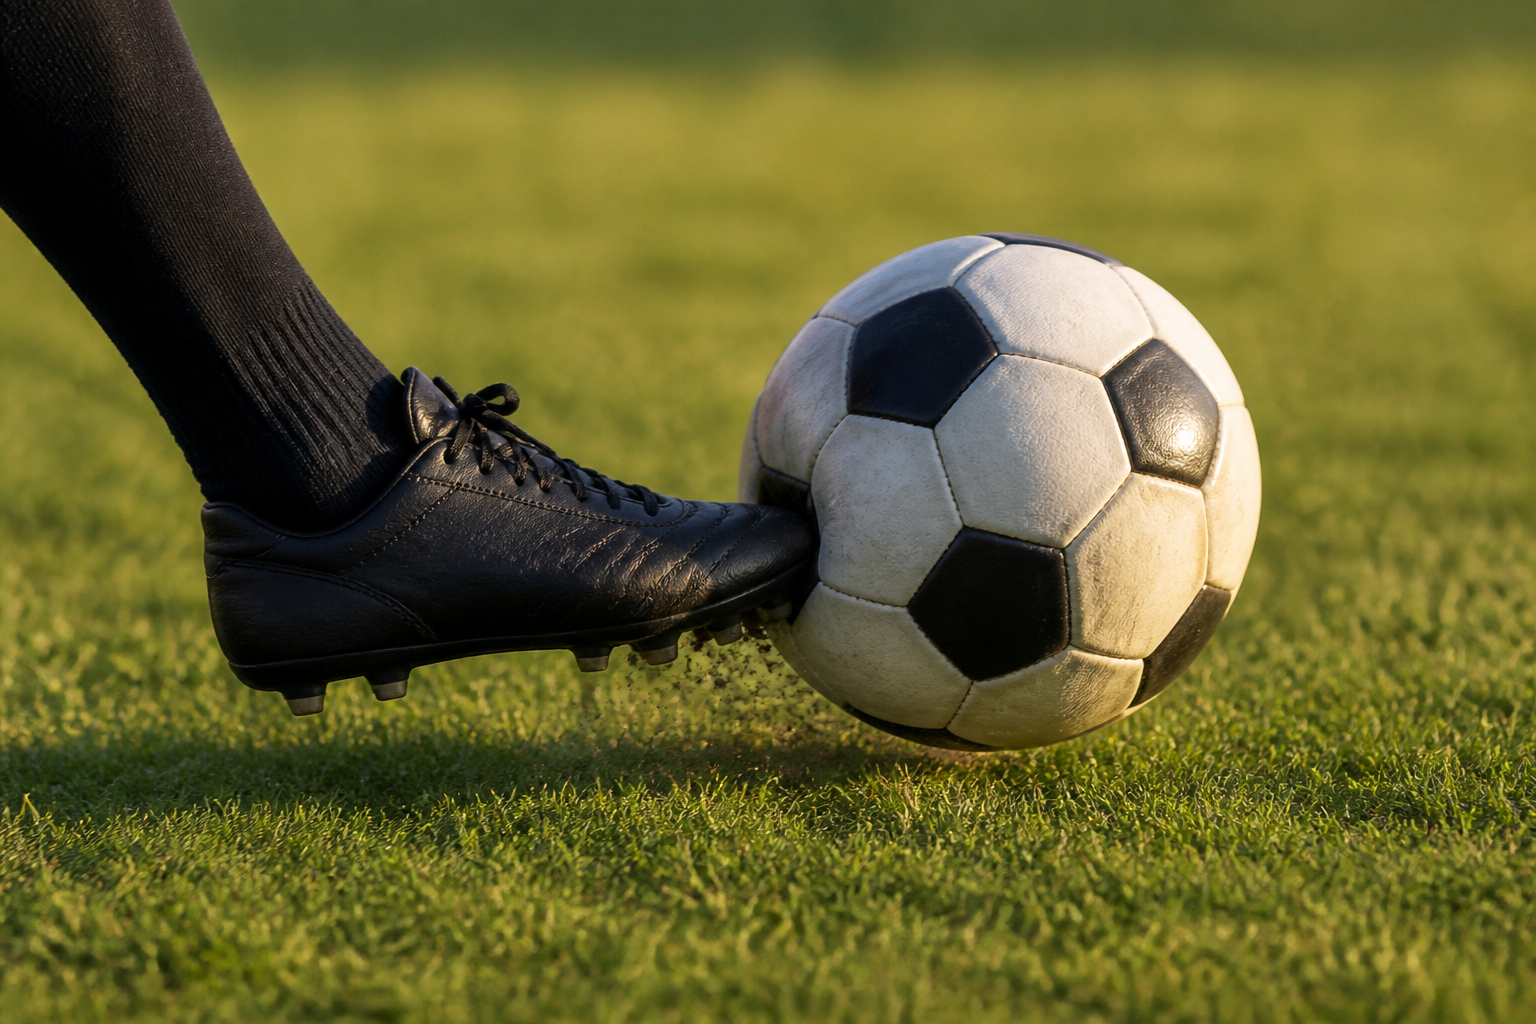
\includegraphics[width=0.58\linewidth]{images/book1/ai/g2-pushes-kick.png}

{\small Una \omterm{def:g2:pushes-and-pulls:force}{fuerza} en el instante en que actúa: la bota empuja y el balón parado está a punto de salir volando.}
\end{omfigure}

\section{Qué hacen las fuerzas}

\begin{proposition}[Los cuatro oficios de una fuerza]\label{prop:g2:pushes-and-pulls:jobs}
Una \omterm{def:g2:pushes-and-pulls:force}{fuerza} puede hacerle cuatro cosas a un objeto:
\begin{enumerate}
  \item \emph{ponerlo} en movimiento --- el chut manda lejos el balón
        parado;
  \item \emph{pararlo} --- las manos del portero paran el disparo;
  \item \emph{desviarlo} --- un toque de lado tuerce el camino del
        balón que rueda;
  \item \emph{cambiarle la forma} --- al apretarla se aplasta la
        esponja, al tirar de ella se estira la goma.
\end{enumerate}
Sin \omterm{def:g2:pushes-and-pulls:force}{fuerza}, ninguna de las cuatro: un objeto al que se deja
completamente en paz sigue haciendo exactamente lo que estaba
haciendo.
\end{proposition}

\begin{omfigure}
\begin{tikzpicture}[scale=0.85]
  \draw[dashed, omExo] (0,0.6) -- (4.2,0.6);
  \fill[omDef] (0.6,0.6) circle (0.24);
  \fill[omDef, opacity=0.45] (3.0,0.6) circle (0.24);
  \draw[-Stealth, very thick, omThm] (4.2,0.6) -- (6.0,1.7);
  \fill[omDef, opacity=0.45] (5.4,1.33) circle (0.24);
  \draw[-Stealth, thick, omThm] (4.2,-0.35) -- (4.2,0.5);
  \node[below, font=\small, omThm] at (4.2,-0.5) {toque de lado aquí};
  \node[below, font=\small] at (1.4,0.3) {rodando recto};
  \node[right, font=\small] at (5.85,2.05) {¡nueva dirección!};
\end{tikzpicture}

{\small El oficio número tres: una pelota que rueda recibe un toque de
lado y su camino se tuerce hacia el empujón.}
\end{omfigure}

\begin{example}[Más fuerza, más efecto]\label{ex:g2:pushes-and-pulls:stronger}
Da un toquecito a una canica: rueda perezosa hasta el borde de la
mesa. Dale un capirotazo fuerte: sale volando por la habitación. La
misma canica, el mismo dedo --- solo ha cambiado la intensidad del
empujón, y el vuelo de la canica ha cambiado con ella. \omterm{def:g2:pushes-and-pulls:force}{Fuerza} suave,
efecto suave; \omterm{def:g2:pushes-and-pulls:force}{fuerza} tremenda, efecto tremendo.
\end{example}

\begin{example}[Pruébalo: los que cambian de forma]\label{ex:g2:pushes-and-pulls:shape}
Reúne una esponja, una goma elástica, un trozo de plastilina y un
taco de madera. Aprieta y estira cada uno. La esponja recupera su
forma en cuanto la sueltas; la goma también. La plastilina se queda
con su forma nueva --- tu \omterm{def:g2:pushes-and-pulls:force}{fuerza} le ha hecho una marca para siempre.
¿Y el taco? Tu apretón más fuerte no lo cambia nada (¡nada que se
pueda ver!). Cada cosa responde a la fuerza a su manera.
\end{example}

\section{Fuerzas sin tocar}

\begin{example}[El tirón de la Tierra]\label{ex:g2:pushes-and-pulls:earthpull}
Suelta una cuchara: se va abajo. Lanza una pelota todo lo alto que
quieras: vuelve abajo. Las hojas, las gotas de lluvia, las migas ---
todo lo que se suelta cae \emph{hacia abajo}. Algo tira de todas y
cada una de esas cosas, todo el rato y sin tocarlas: la propia Tierra.
El tirón de la Tierra es la \omterm{def:g2:pushes-and-pulls:force}{fuerza} más constante de tu vida --- no
suelta nunca, y por eso ``abajo'' significa lo mismo en todos los
rincones del patio.
\end{example}

\begin{omfigure}
\begin{tikzpicture}[scale=0.85]
  % the falling apple
  \draw[thick] (0,0) -- (5.0,0);
  \draw[thick, red!60!black, fill=red!70] (1.4,2.5) circle (0.32);
  \draw[thick, brown!60!black]
    (1.4,2.82) .. controls (1.45,2.98) .. (1.56,3.08);
  \draw[thick, green!45!black, fill=green!45]
    (1.62,3.02) ellipse [x radius=0.16, y radius=0.07, rotate=30];
  \draw[-Stealth, very thick, omDef] (1.4,2.05) -- (1.4,1.1);
  \node[right, font=\small, omDef] at (1.65,1.6)
    {la Tierra tira hacia abajo};
  \node[below, font=\small] at (2.5,-0.25)
    {la manzana cae: tirada, no empujada};
  % the magnet holding a paperclip up across a gap
  \draw[thick, fill=red!70] (7.9,2.35) rectangle (8.75,2.95);
  \draw[thick, fill=blue!60] (8.75,2.35) rectangle (9.6,2.95);
  \begin{scope}[shift={(8.54,1.65)}, rotate=-90]
    \draw[thick, rounded corners=2.6pt]
      (0,0) -- (1.1,0) -- (1.1,0.42) -- (0.12,0.42) -- (0.12,0.14)
      -- (0.95,0.14) -- (0.95,0.30) -- (0.30,0.30);
  \end{scope}
  \draw[-Stealth, very thick, omDef] (9.15,1.0) -- (9.15,2.0);
  \node[below, font=\small] at (8.75,0.1)
    {el imán tira hacia arriba --- sin tocar};
\end{tikzpicture}

{\small Dos \omterm{def:g2:pushes-and-pulls:force}{fuerzas} que no tocan: la Tierra tira de la manzana hacia
abajo a través del \omterm{def:g2:air-around-us:air}{aire}; el \omterm{def:g1:magnets:magnet}{imán} tira del clip hacia arriba a
través del \omterm{def:g2:air-around-us:air}{aire}.}
\end{omfigure}

\begin{remark}[Viejos conocidos]\label{rem:g2:pushes-and-pulls:magnets}
Ya conoces otra \omterm{def:g2:pushes-and-pulls:force}{fuerza} que no toca: el \omterm{def:g1:magnets:magnet}{imán}, tirando de su clip a
través de un hueco de \omterm{def:g2:air-around-us:air}{aire}. Los imanes y el tirón de la Tierra son
las dos \omterm{def:g2:pushes-and-pulls:force}{fuerzas} sin contacto de tu vida diaria --- excepciones raras
y preciosas, porque cualquier otro empujón o tirón con el que te
cruces necesita tocar. Las dos crecerán hasta convertirse en grandes
capítulos más adelante en este curso.
\end{remark}

\section{Ejercicios}

\begin{exercise}[$\star$]\label{exo:g2:pushes-and-pulls:1}
¿Empujón o tirón? Llamar a un timbre; \ abrir un cajón; \ rematar de
cabeza un balón; \ arrastrar un trineo cuesta arriba; \ apretar el
tubo de pasta de dientes.
\end{exercise}

\begin{exercise}[$\star$]\label{exo:g2:pushes-and-pulls:2}
¿Qué tres cosas cuenta sobre una \omterm{def:g2:pushes-and-pulls:force}{fuerza} la flecha que la representa?
\end{exercise}

\begin{exercise}[$\star$]\label{exo:g2:pushes-and-pulls:3}
Nombra los cuatro oficios de una \omterm{def:g2:pushes-and-pulls:force}{fuerza} y pon un ejemplo tuyo de cada
uno --- distinto de los del capítulo.
\end{exercise}

\begin{exercise}[$\star$]\label{exo:g2:pushes-and-pulls:4}
Una canica rueda derecha hacia ti. Usando solo un dedo, ¿cómo haces
que: se pare; \ vaya más deprisa; \ se desvíe hacia un lado? Di hacia
dónde empuja tu dedo cada vez.
\end{exercise}

\begin{exercise}[$\star$]\label{exo:g2:pushes-and-pulls:5}
¿Cuáles recuperan su forma y cuáles se quedan con la marca: una
esponja; \ la plastilina; \ una goma elástica; \ la nieve blanda?
\end{exercise}

\begin{exercise}[$\star$]\label{exo:g2:pushes-and-pulls:6}
Dibuja una caja empujada suavemente hacia la derecha y la misma caja
empujada con fuerza hacia la izquierda. ¿En qué se diferencian tus dos
flechas?
\end{exercise}

\begin{exercise}[$\star$]\label{exo:g2:pushes-and-pulls:7}
¿Qué \omterm{def:g2:pushes-and-pulls:force}{fuerza} hace caer todo lo que se suelta? ¿Necesita tocar la
cuchara que cae? ¿Hacia dónde tira siempre?
\end{exercise}

\begin{exercise}[$\star$]\label{exo:g2:pushes-and-pulls:8}
Di las dos \omterm{def:g2:pushes-and-pulls:force}{fuerzas} sin contacto que has conocido, cada una con un
ejemplo visto en casa.
\end{exercise}

\begin{exercise}[$\star\star$]\label{exo:g2:pushes-and-pulls:9}
En el juego de tirar de la cuerda, los dos equipos tiran con todas sus
\omterm{def:g2:pushes-and-pulls:force}{fuerzas} y, sin embargo, la cinta atada a la soga a veces no se mueve
nada. Dibuja la soga con las flechas de los dos equipos. ¿Qué tiene que pasar con
los dos tirones para que la cinta se quede quieta? ¿Qué ocurre en el
momento en que un equipo tira más fuerte?
\end{exercise}

\begin{exercise}[$\star\star$]\label{exo:g2:pushes-and-pulls:10}
Una pelota lanzada recta hacia arriba va frenando, se para un abrir y
cerrar de ojos y vuelve a caer. ¿Qué \omterm{def:g2:pushes-and-pulls:force}{fuerza} está actuando durante la
subida, arriba del todo y durante la bajada? ¿Deja de tirar en algún
momento? (Dibuja la flecha en cada uno de los tres instantes.)
\end{exercise}
